% Template for ISBI-2018 paper; to be used with:
%          spconf.sty  - ICASSP/ICIP LaTeX style file, and
%          IEEEbib.bst - IEEE bibliography style file.
% --------------------------------------------------------------------------
\documentclass{article}
\usepackage{spconf,amsmath,graphicx}

% Example definitions.
% --------------------
\def\x{{\mathbf x}}
\def\L{{\cal L}}

% Title.
% ------
\title{Scoliosis Screening and Monitoring using Self Contained Ultrasound and Neural Networks}
%
% Single address.
% ---------------
\makeatletter
\def\@name{ \emph{Hastings Greer, Sam Gerber, Marc Niethammer, Roland Kwitt},  \\ \emph{Matt McCormick, Deepak Chittajallu, Neal Siekierski, Stephen Aylward}}
\makeatother
%\name{Hastings Greer  Sam Gerber, Marc Niethammer, Roland Kwitt,
%Matt McCormick, Deepak Chittajallu, Neal Siekierski, Stephen Aylward }
\address{Kitware Inc\\
Carrboro NC 27510, USA}
%
% For example:
% ------------
%\address{School\\
%	Department\\
%	Address}
%
% Two addresses (uncomment and modify for two-address case).
% ----------------------------------------------------------
%\twoauthors
%  {A. Author-one, B. Author-two\sthanks{Thanks to XYZ agency for funding.}}
%	{School A-B\\
%	Department A-B\\
%	Address A-B}
%  {C. Author-three, D. Author-four\sthanks{The fourth author performed the work
%	while at ...}}
%	{School C-D\\
%	Department C-D\\
%	Address C-D}
%
% More than two addresses
% -----------------------
% \name{Author Name$^{\star \dagger}$ \qquad Author Name$^{\star}$ \qquad Author Name$^{\dagger}$}
%
% \address{$^{\star}$ Affiliation Number One \\
%     $^{\dagger}$}Affiliation Number Two
%
\begin{document}
%\ninept
%
\maketitle
%
\begin{abstract}
We aim to diagnose scoliosis using a self contained ultrasound device that does not require significant training to operate. The device knows its angle relative to vertical using an embedded inertial measurement unit, and it estimates its angle relative to a vertebrae using a neural network analysis of its ultrasound images.  The composition of those angles defines the angle of a vertebrae from vertical.  The maximum difference between vertebrae angles collected from a scan of a spine yields the Cobb angle measure that is used to quantify scoliosis severity. 
\end{abstract}
%
\begin{keywords}
Point-of-Care Ultrasound, Computer Aided Diagnosis
\end{keywords}
%
\section{Introduction}
\label{sec:intro}

Scoliosis is a complex three-dimensional deformity characterized primarily by lateral curvature and rotational deviation of the spine. Different types of scoliosis exist, including congenital, neuromuscular, and syndromic; and the most common is idiopathic, which affects otherwise healthy children. The prevalence of idiopathic scoliosis ranges from 0.5\% to 3\% \cite{Mor06} with 2-4\% of children ages 6 to 14 having pathologic spinal curves greater than 20\%. The most significant risk factor for curve progression is growth, with children entering their adolescent growth spurts at particular risk. While children and adults can live relatively symptom free with small scoliotic curves, as these curves increase in size, the risk of health problems increases concurrently. Surgery is typically recommended for curves over 50$^\circ$. With curves over 75-80$^\circ$, significant disability due to restrictive pulmonary and cardiac disease can occur \cite{Hae06}.
"
Our system is targeting scoliosis screening the general population and quantitatively monitoring scoliosis progression in known cases. As such, our system is intended to be used in the field: at schools, in the offices of general practitioners, and in the offices of pediatric orthopedic surgeons.

\subsection{Screening}
\label{ssec:screen}
Many states in the USA mandate school screening for scoliosis. In general, a scoliometer is used to assess the rotational deformity of a child's back. Children with scoliometer measurements greater than 5$^\circ$ are referred for further evaluation. X-ray imaging is then typically used. Unfortunately, a scoliometer is quite insensitive and non-specific. It has been reported that the positive predictive value of a scoliometer reading of 5$^\circ$ to detect real scoliosis is only 4\% \cite{Yaw99}. This results in a large number of unnecessary referrals to physicians and unneeded X-rays of developing children.

\subsection{Monitoring}
\label{ssec:Monitoring}
 The most common method for monitoring scoliosis is to measure the spinal curvature using Cobb's method \cite{Cob48} from posteroanterior (PA) X-Ray images. A minimum of 10$^\circ$ of Cobb angle is needed to differentiate scoliosis.  However, radiographs are costly and expose children to potentially harmful ionizing radiation. It is estimates that children with scoliosis progression undergo three to seven x-ray images per year, and such radiation exposure increases the risk of leukemia, lung cancer, and breast cancer. \cite{Kno14}
 
There has been extensive research into replacing scoliometers and X-Ray imaging with computer-assisted ultrasound imaging systems to reduce costs, increase reliability, and eliminate the need for harmful radiation \cite{Li10, Che13, Ung14a}.  However, most of the ultrasound research systems (1) require the use of external tracking equipment, (2) rely on the operator or an advanced algorithm to precisely locate key landmarks in the ultrasound data, and/or (3) do not provide real-time guidance to the operator, so the operators must still be trained to capture usable scans.  Great progress has been made to tackle each of these challenges, and promising results are being generated (\cite{Che13, Ung14a} have reported approximately 2$^\circ$ difference compared to radiographs), but we have chosen to explore a self-contained ultrasound-based solution that eliminates the need for external tracking, landmark identification, or extensive operator training.

Our system is based on ultrasound imaging, but an ultrasound image is never presented to the operator.  The operator must be trained regarding how to apply sufficient acoustic gel and how to move the device so as to follow the spine of a child, but the embedded image analysis algorithms and the embedded graphic display provide simple feedback to the operator to ensure that sufficient acoustic gel has been used and that the probe remains over the spine as it is moved.  After a sweep has been completed, the device displays the estimated Cobb angle.

The methods section describes the image analysis and deep learning methods employed by our device.  The experiment section presents results using a spine phantom then indicate that our device can produce results that are more accurate than a scoliometer and nearly as accurate as X-ray imaging.  This paper concludes with a discussion of future steps for device research, development, and validation.

\section{Methods}
\label{sec:methods}

Instead of requiring challenging intermediate steps such as externally tracking an ultrasound probe using optical technologies, reconstructing an ultrasound volume from tracked 2D ultrasound images, determining the coordinates of key landmarks, or registering a volume to an atlas, our system directly estimates the angle between the spine and the ultrasound probe using a neural network. In combination with an internal inertial measurement unit (IMU) to report the angle between the ultrasound probe and vertical, our self-contained, hand-held unit bypasses the traditional intermediate steps and focuses on the measures to be made. The Cobb Angle is defined by the extrema of the estimated angles.

The input training data comes from ultrasound image sequences taken of a model spine immersed in water. The ideal output training data for that input training data is the orientation of the ultrasound probe along each sequence, as measured using an optical tracker.  All training data is accomplished with the model spine straightened, which is sufficient since the neural network only needs to estimate the angle between the ultrasound probe and the underlying vertebrae. The probe is swept up and down the spine while simultaneously rotated along the coronal axis, to obtain 170,000 training images. The ultrasound data is passed to the neural network as B-mode images that have been scaled down to 100x100, and augmented by flipping over the vertical axis.

\begin{figure}
\centering
\begin{tabular}{cc}
\centering
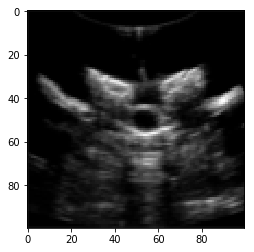
\includegraphics[height=5.5cm,keepaspectratio]{SampleInput}
\end{tabular}
\caption{A sample frame, as passed to the network
}
\end{figure}


Our system's neural network consists of two parts. A convolutional network modeled after VGG processes each frame, and is trained to predict the angle given a single frame. Then, this network has its last layer removed, and the remainder is used to pre-process each frame. Finally, a second fully connected network processes a sliding window of 41 pre-processed frames, stacked into an unstructured vector.

\begin{table}[ht]
\caption{Convolutional Network}
\begin{tabular}{c c c c c}
\hline \\
Type & \# Filters & Stride & Activation & Rate \\
\hline
Convolution & 32 & 3x3 & Relu \\
Max Pooling &    & 2x2 &      \\
Convolution & 64 & 3x3 & Relu \\
Max Pooling &    & 2x2 &      \\
Convolution & 64 & 3x3 & Relu \\
Max Pooling &    & 2x2 &      \\
Convolution &128 & 3x3 & Relu \\
Convolution &256 & 3x3 & Relu \\
Fully Connected & 512 & & Relu \\
Dropout & & & & 0.5 \\
Fully Connected & 512 & & Relu \\
Dropout & & & & 0.5 \\
Fully Connected & 1 & & tanh \\
\end{tabular}
\end{table}

\begin{table}[ht]
\caption{Sliding Window Network}
\begin{tabular}{c c c}
\hline \\
Type & \# Filters & Activation \\
\hline
Fully Connected & 1024  & Relu \\
Fully Connected & 1024  & Relu \\
Fully Connected & 1 &  tanh \\
\end{tabular}
\end{table}

Once the network has been trained, the vertebrae-to-probe angle given by the neural network is subtracted from the probe-to-vertical angle given by the accelerometer embedded in the ultrasound probe. The resulting vertebrae-to-vertical angle sequence is then smoothed with a median filter, and the difference between the maximum and minimum estimated vertebrae-to-vertical angles is the computed Cobb angle.   

\section{Experiment and Results}

As a preliminary validation, we tested our network’s ability to deduce the angle of the ultrasound probe on images of a straight spine acquired while rotating the ultrasound probe as it moved down the spine.  This testing data was captured after (i.e., completely separate from) the training data and consisted of 10,000 images. Our results on this data are shown in fig. 2. For the smoothed data, the mean error is 2.0 degrees, the standard deviation is 3.7 degrees, and the 95th percentile error is 5.8 degrees. 

\begin{figure}
\centering
\begin{tabular}{c}
\centering
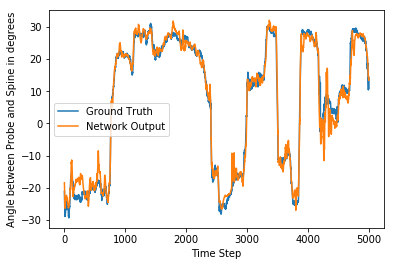
\includegraphics[height=5.5cm,keepaspectratio]{NetworkOutput} 

\end{tabular}
\begin{tabular}{c}
\centering

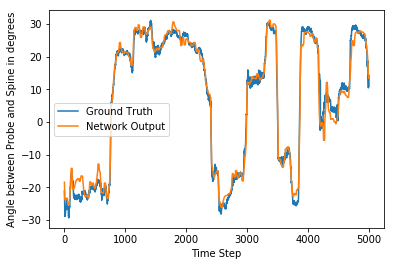
\includegraphics[height=5.5cm,keepaspectratio]{MedFilterNetworkOutput}
\end{tabular}
\caption{Graph of estimated and actual ultrasound probe angle as the probe is moved and rotated along a spine, for testing data.  Top graph: raw network predictions.  Bottom graph: median filter applied to the predictions.  The neural network estimates this angle using only the image data.  At transitions between vertebrae and at time step 4300, the angle measures temporarily degrade, but otherwise, the estimated and actual angles are typically within +/- 2$^\circ$.  The full system applies median filtering to these data to eliminate local irregularities.
}
\end{figure}
 
\section{Automated Operator Guidance}
We anticipate that in order to function with no operator training, our system will need to guide the operator to keep the spinal column visible in the ultrasound image. To that end, we also trained a neural network
to predict the lateral position of the probe with respect to the spine from the image data. This network used the same architecture as was used to predict the vertebral angles from a single image frame. In inference mode this network runs faster than real time and is sufficiently accurate to provide feedback to the operator such as "Move Right," "Move Left," or "You are Centered." We intend to display this guidance as arrows on the screen of the final product.  Figure 3 shows the correlation between the network's estimate of probe offset from center relative to the probes actual offset as measured via an external tracker.  For the majority of the scans, the neural network estimates would correctly guide the user to keep the ultrasound probe within the 2.5cm margin needed to keep the spine fully within the ultrasound image's field of view. The system also correctly identifies when the spine has move out of the required range for the majority of conditions.

\begin{figure}
\centering
\begin{tabular}{cc}
\centering
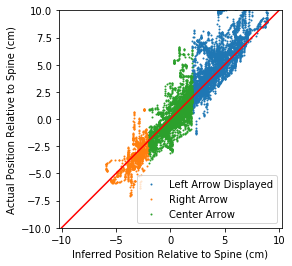
\includegraphics[height=7.4cm,keepaspectratio]{Guidance}
\end{tabular}
\caption{A neural network infers whether the operator needs to move the probe to the left or right to stay centered on the spine
}
\end{figure}

\section{Discussion and Future Work}
The system design provides a self-contained ultrasound device that can estimate Cobb angle to screen and monitor scoliosis.  One neural network is able to estimate the angle between an ultrasound probe and a vertebral body within 2$^\circ$, while another neural network provides feedback to the user to keep the vertebral bodies centered within the ultrasound field of view.  

For future work, we intend to include information from the guidance network when deciding which frames to take into account. Currently, testing frames where it is not possible to deduce the correct angle due to operator error count against our program. The finished system must be able to discard frames that it cannot interpret, instead of making a bad guess. If too many frames are unusable, the system should demand a re-sweep and refuse to estimate a Cobb Angle.

We also anticipate that a more structured neural network architecture could improve accuracy. In particular, it is unusual that post processing  with a median filter improves results, given that a sufficiently complex network should be able to learn to smooth its output. 

Finally, we anticipate that better training data could be obtained by annotating the position and angle of each vertebra in the phantom individually, instead of straightening a spine and then defining the global rotation of each vertebra to be 0. Any bend in the training spine becomes error that the network can never learn. Individual annotation would also allow us to include bent spines in the training data.

We aim to operate this software on our planned hand held, self contained ultrasound device. This device, which runs off of an Intel compute stick and windows 10, will enable an extremely simple and fast workflow, where the operator sweeps the device over the patient’s back, following the onscreen arrows to keep centered on the spine, and then reads the cobb angle off of the screen. Because the device runs the same windows version as the computers we are currently running our research on, we do not anticipate any difficulty in porting to the new platform.

\bibliographystyle{IEEEbib}
\begin{thebibliography}{}
%
\bibitem[1]{Mor06}
RT. Morrissy, and SL. Weinstein, �Idiopathic Scoliosis in Lovell and Winter�s Pediatric Orthopedics,� Lippincott Williams and Wilkins, Philadelphia, 2006, pp. 694-762.

\bibitem[2]{Hae06}
M. Haefeli, A. Elfering, R. Kilian, K. Min and N. Boos "Nonoperative treatment for adolescent idiopathic scoliosis: a 10- to 60-year follow-up with special reference to health-related quality of life." Spine (Phila Pa 1976), 31(3): 355-66; discussion 367, 2006

\bibitem[3]{Yaw99}
BP. Yawn, RA. Yawn, D. Hodge, M. Kurland, WJ. Shaughnessy, D. Llstrup, and SJ. Jacobsen, "A population based study of school scoliosis screening." JAMA, 282(15): 1427-32, 1999.

\bibitem[4]{Cob48}
J. Cobb, �Outline for the Study of Scoliosis,� Instructional Course Lectures, Vol. 5, 1948, pp. 261-275. 

\bibitem[5]{Kno14}
P. Knott, E. Pappo, M. Cameron, JC. deMauroy, et al., "SOSORT 2012 consensus paper: reducing x-ray exposure in pediatric patients with scoliosis" Scoliosis 2014, 9:4

\bibitem[6]{Li10}
M. Li, C. Cheng, M. Ying, et al. "Applications of 3D Ultrasound in Assisting the Fitting Procedure of Spinal Orthosis to Patients with Adolescent Idiopathic Scoliosis,� Studies in Health Technology and Informatics, Vol. 158, 2010, pp. 34-3

\bibitem[7]{Che13}
W. Chen, EH. Lou, P. Zhang, LH. Le, D. Hill. "Reliability of assessing the coronal curvature of children with scoliosis by using ultrasound images", Journal of Children's Orthopaedics, 7(6):521-9, Dec 2013

\bibitem[8]{Ung14a}
T. Ungi, F. King, M. Kempston, Z. Keri, A. Lasso, P. Mousavi, et al.  Spinal curvature measurement by tracked ultrasound snapshots. Ultrasound in Medicine and Biology. 40(2), 2014:447-54.

\end{thebibliography}

\bibliography{strings,refs}

\end{document}
